\chapter{Experimental Design} \label{ch:Exp_Design}

\section{Testing Considerations}

Before venturing further, we should summarize the goals of the UKF framework described previously, paying particular attention to unmanned aircraft system (UAS) operations. This ROS package was designed with the express intent of producing estimates of the position vector $\mathbf{p}$ and orientation quaternion $\mathbf{q}$ of a rotorcraft UAV in real time. Thus, the experiments testing the system's efficacy compare the filter's estimates of position and orientation to the ground truth measured by Vicon.

\begin{figure}[t]
    \centering
    \begin{subfigure}[t]{0.5\textwidth}
        \centering
        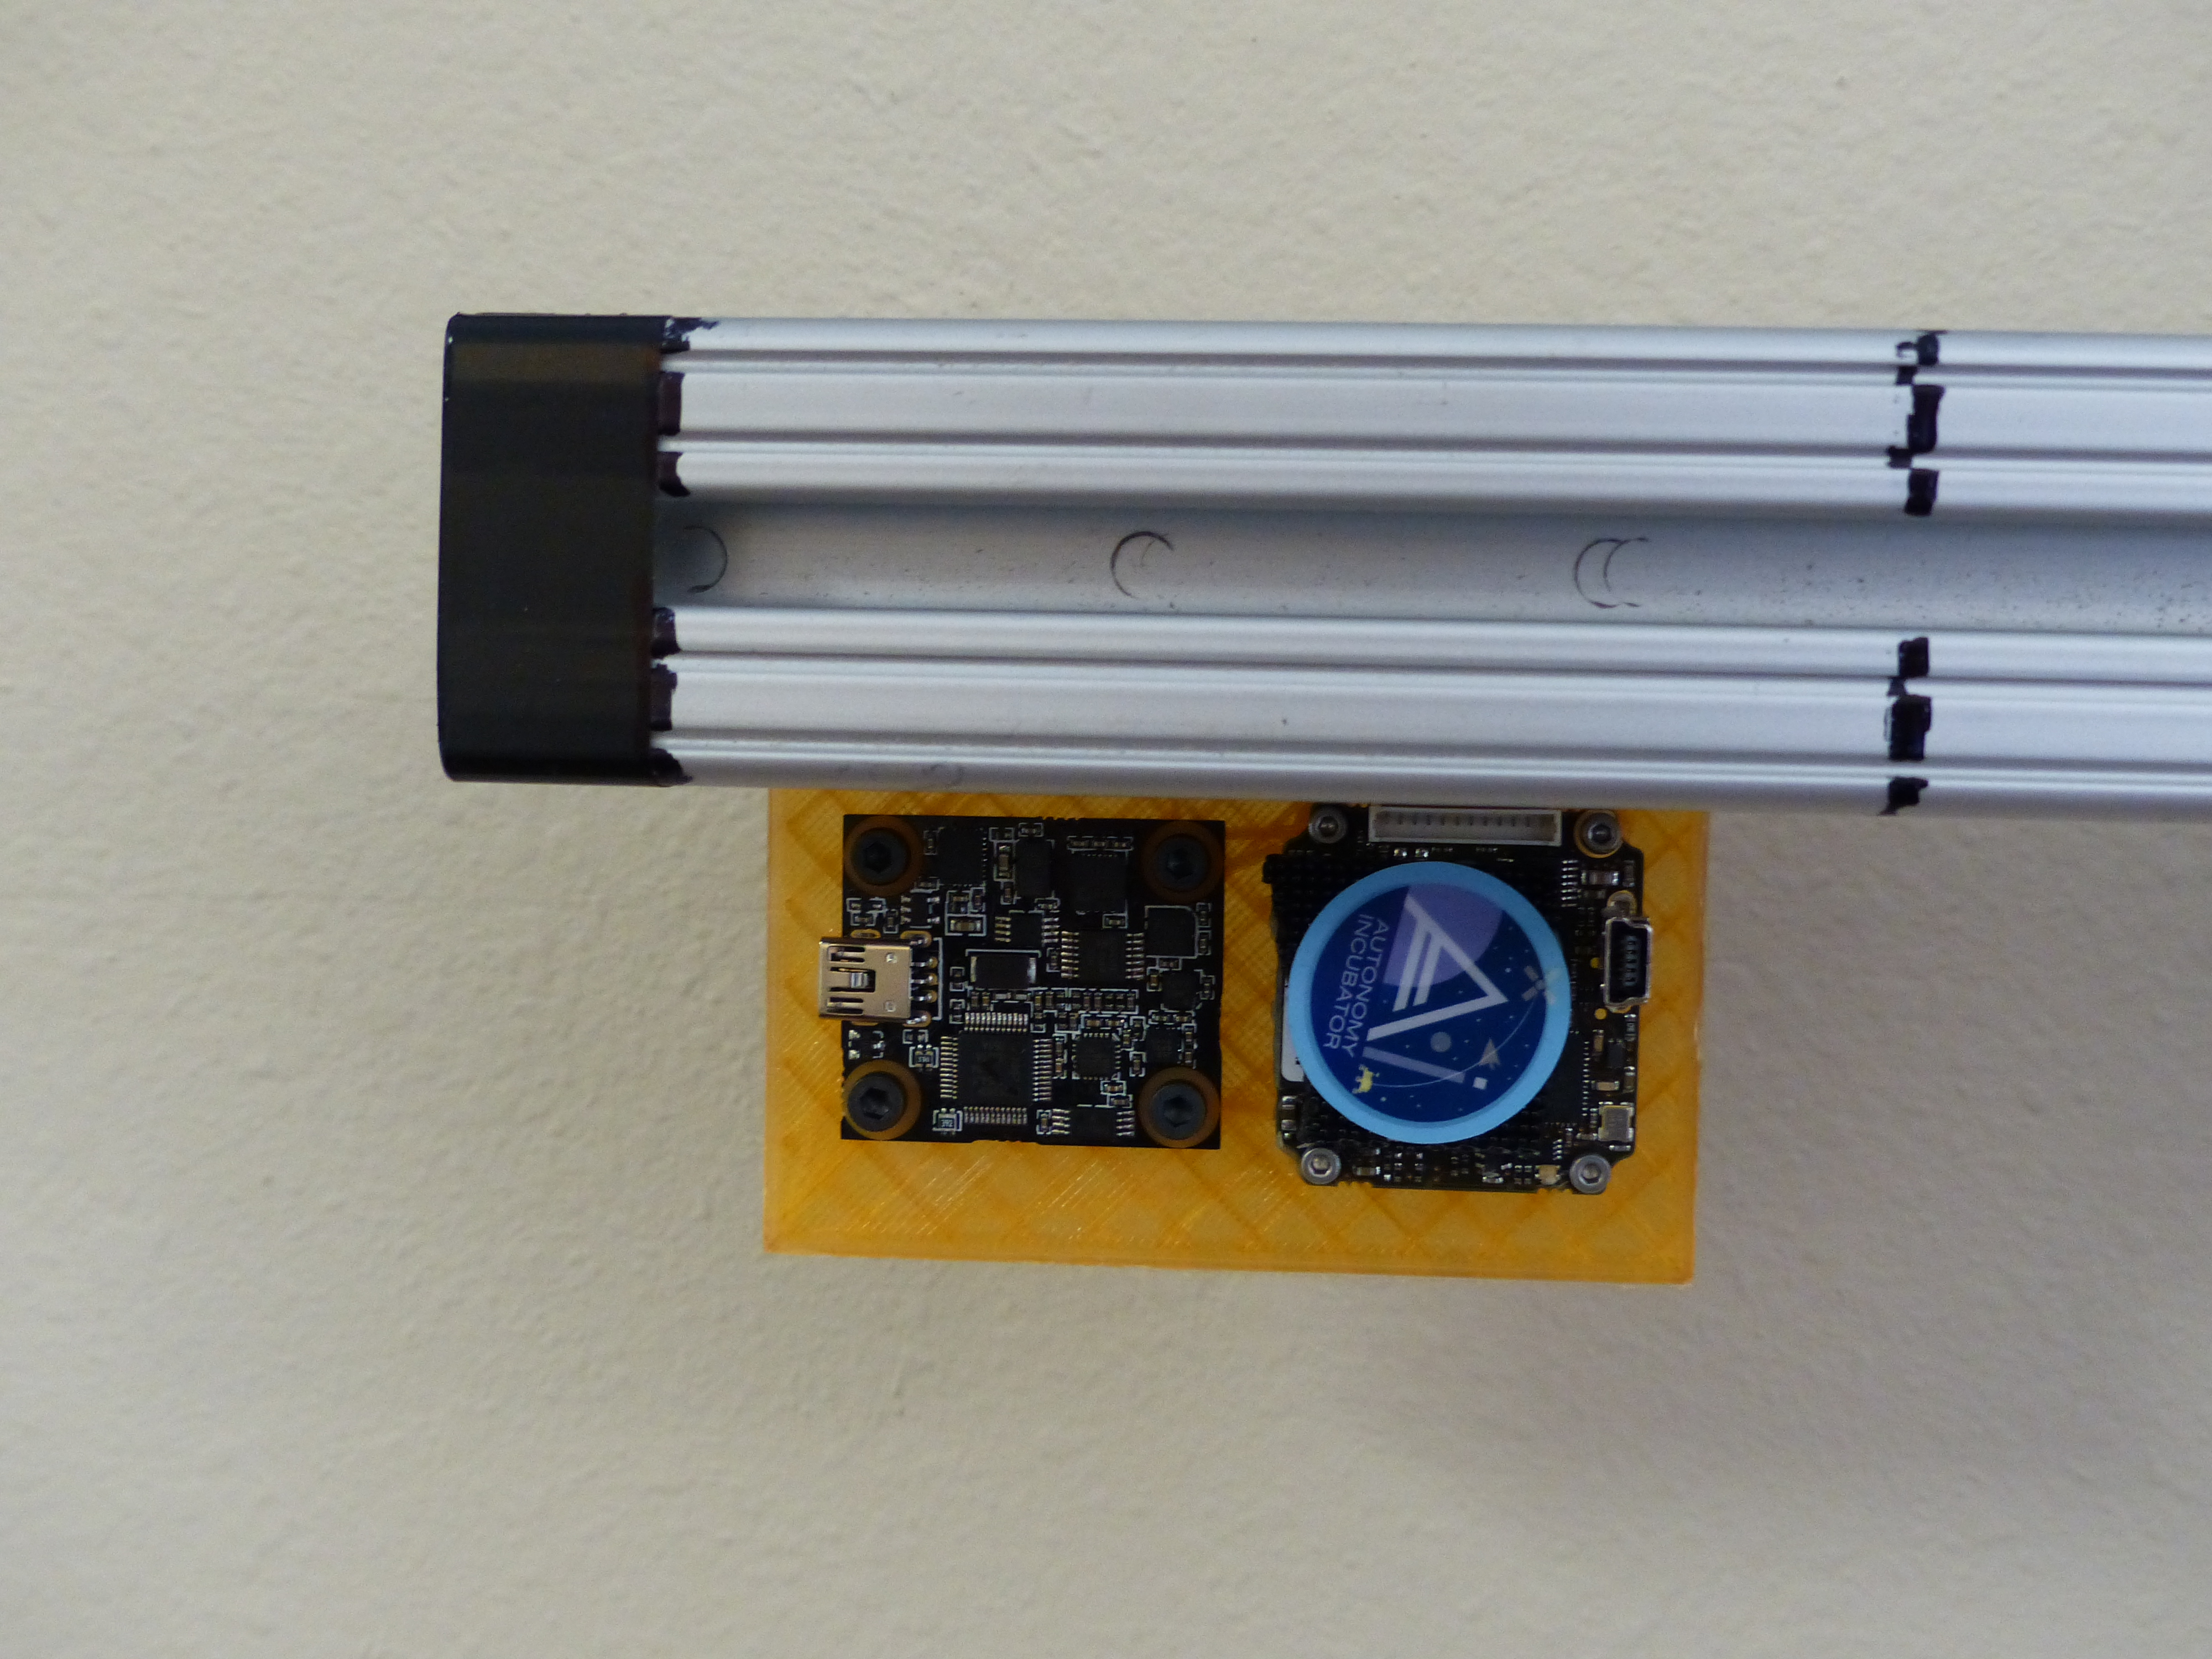
\includegraphics[width=0.8\textwidth]{sensor_mount_top}
        \caption{Top view of sensor mount.}
    \end{subfigure}%
    ~ 
    \begin{subfigure}[t]{0.5\textwidth}
        \centering
        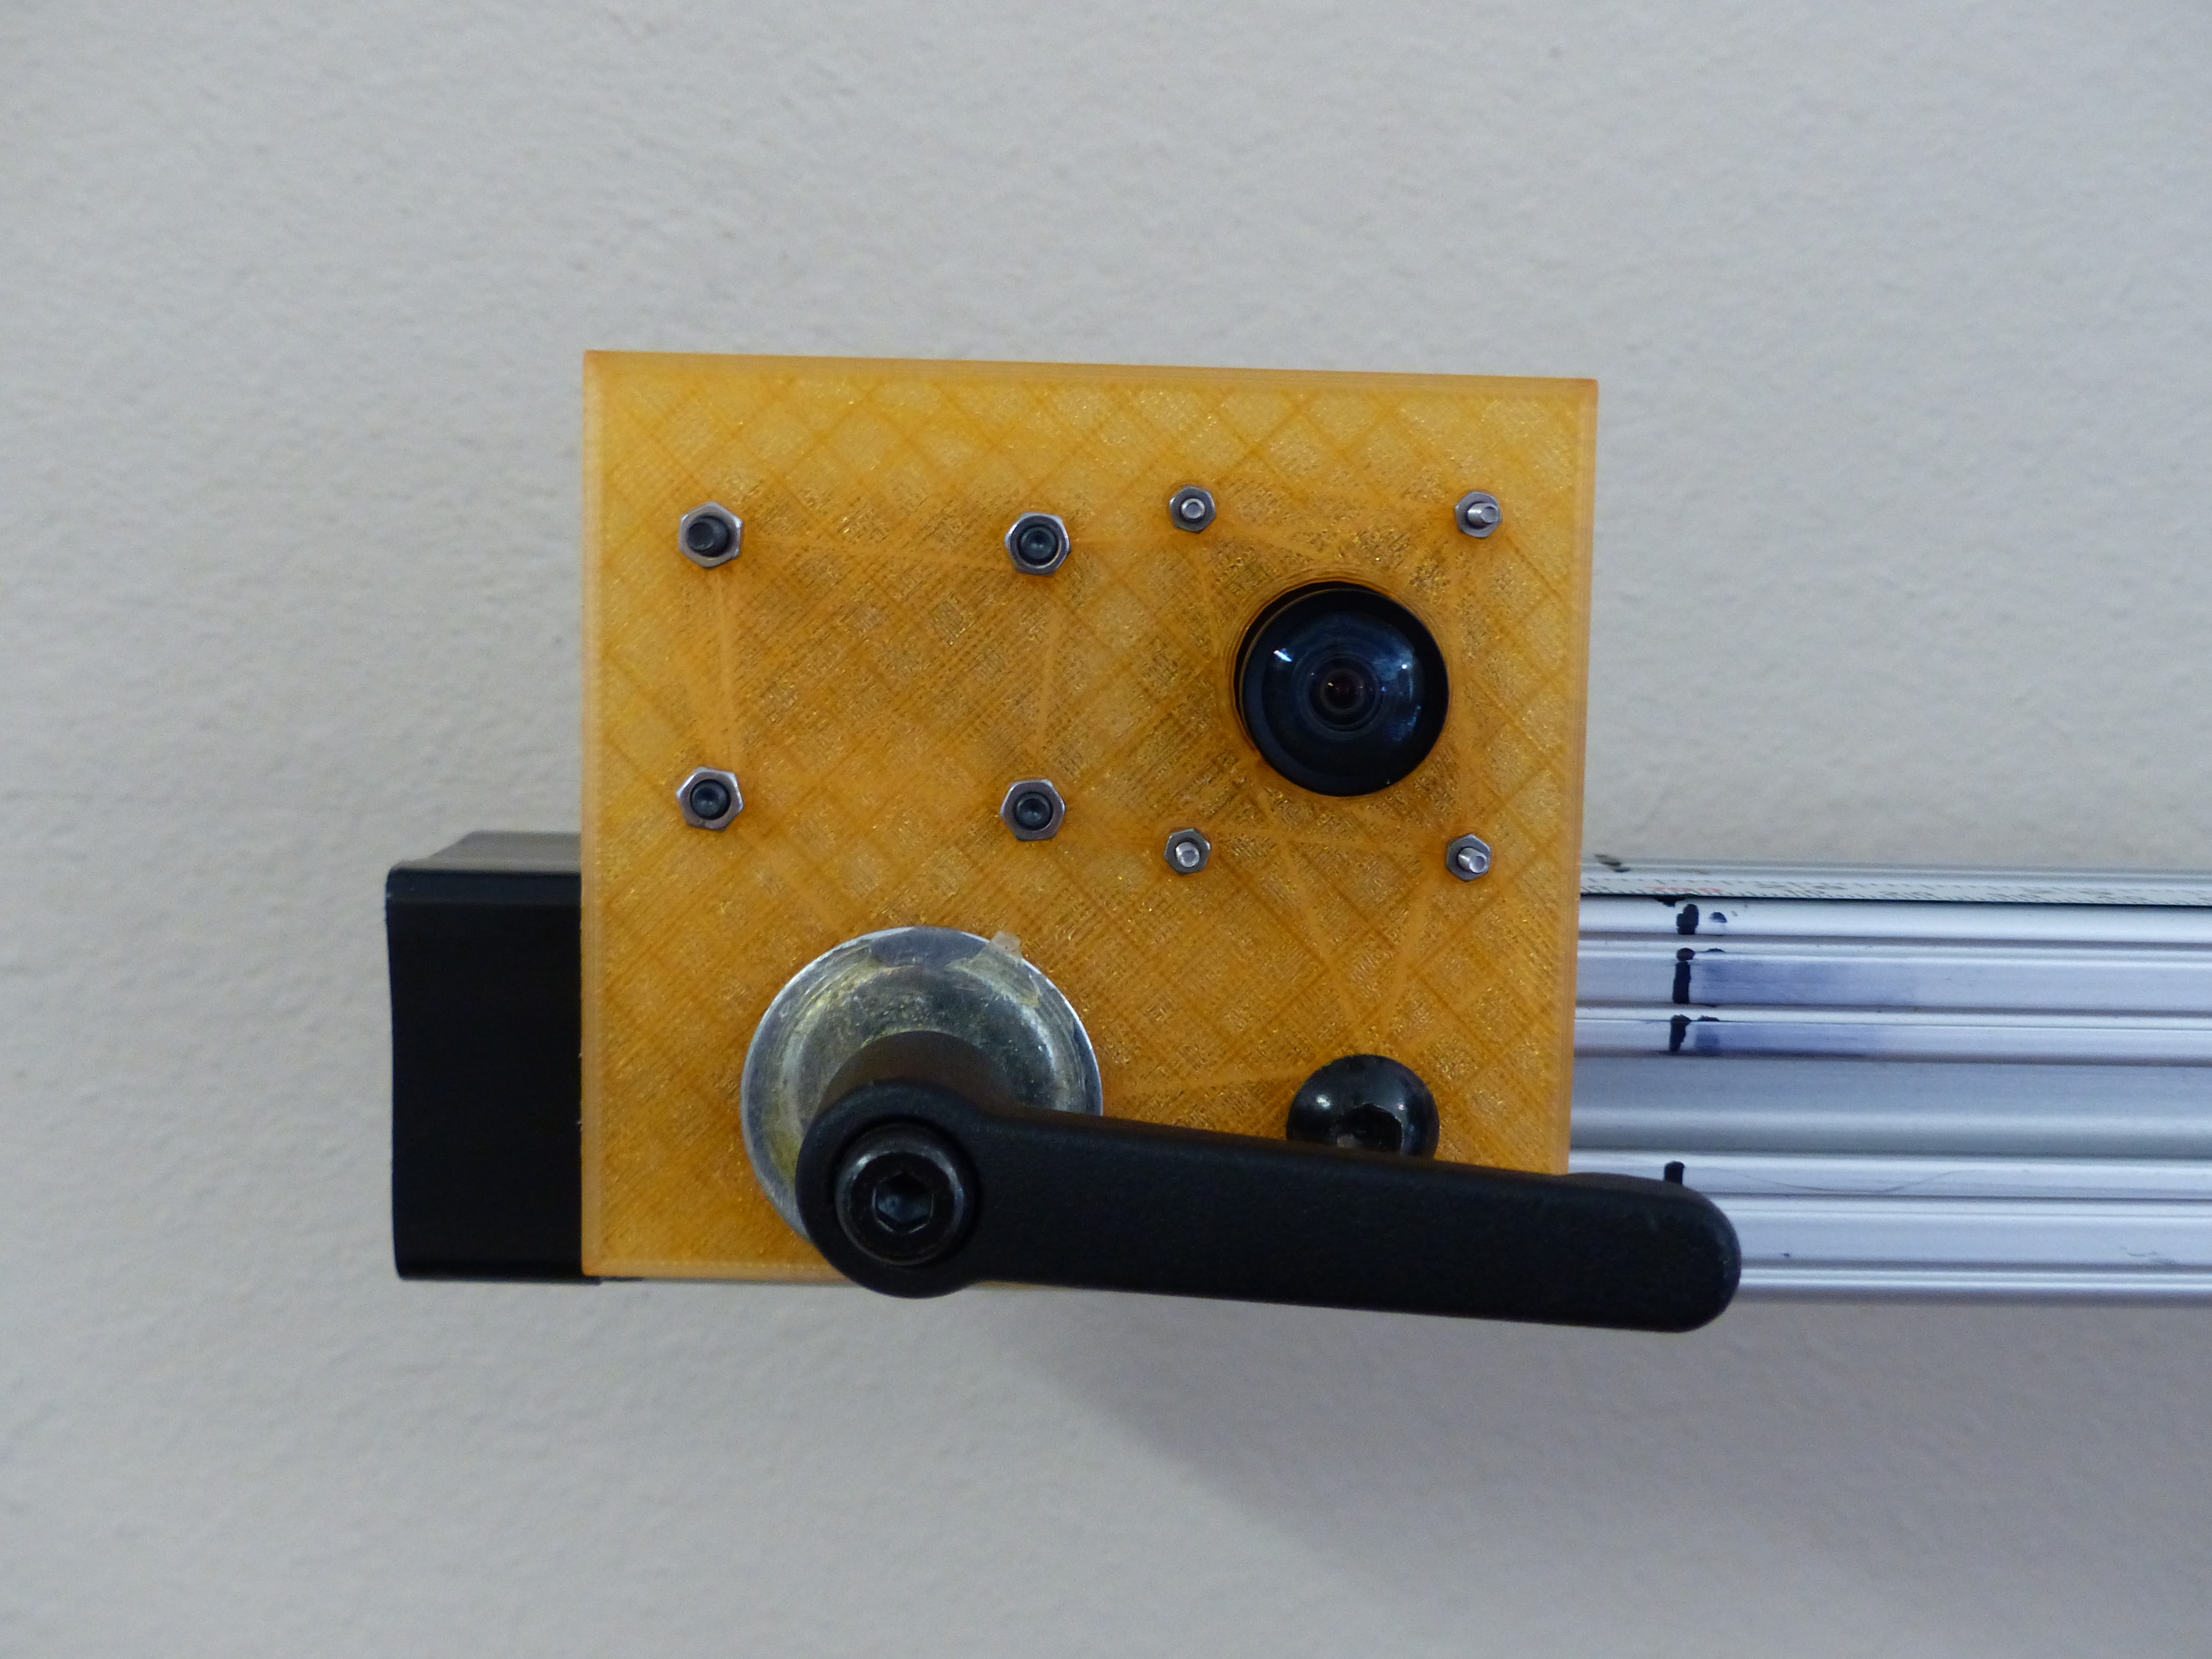
\includegraphics[width=0.8\textwidth]{sensor_mount_bottom}
        \caption{Bottom view of sensor mount.}
    \end{subfigure}
    \caption[3D-printed sensor mount]{The 3D-printed sensor mount. In (a), the Phidgets IMU is on the left and the mvBlueFOX camera is on the right. In (b), the linear braking handle is visible.}
    \label{fig:sensor_mount}
\end{figure}

This system depends upon two sensors: a single global-shutter camera and an IMU. The IMU used in this experiment contains a 3-axis accelerometer and 3-axis gyroscope. To simulate both sensors moving through the scene in a manner reminiscent of hovering rotorcraft flight, a rolling test stand was constructed to carry the sensors safely throughout a large motion capture environment. Mounting the sensor suite on a large, steady, level platform allows for a high degree of control over the accelerations and angular velocities felt by the IMU, as well as the motion captured by the ventral camera. In order to validate the UKF framework's effectiveness under ideal conditions, a modern laptop computer containing an Intel i7 processor with 16~GB of RAM was used for all computations. The floor of the motion capture environment was strewn with a mixture of April tags and modified Quick Response\footnote{\url{https://en.wikipedia.org/wiki/QR_code}} (QR) codes in order to provide sufficient visual features for PTAM to track.

\section{Materials}
\subsection{Computation and Sensing}
\begin{enumerate}
\item One (1) MatrixVision mvBlueFOX-MLC Camera\footnote{\url{https://www.matrix-vision.com/USB2.0-single-board-camera-mvbluefox-mlc.html}}
\item One (1) 1044\_0 PhidgetSpatial Precision 3/3/3 High Resolution IMU\footnote{\url{http://www.phidgets.com/products.php?product_id=1044}}
\item One (1) Hewlett-Packard Spectre x360 Convertible Laptop 13-ac076nr\footnote{\url{http://store.hp.com/us/en/pdp/hp-spectre-x360---13-ac076nr}}
\item Two (2) male Mini USB 2.0 to male USB Type A cables
\end{enumerate}

\subsection{Mobile Test Stand}
\begin{enumerate}
\item One (1) Oklahoma Sound PRC200 Premium Presentation Cart\footnote{\url{http://www.oklahomasound.com/products/product-category/single/?prod=9}}
\item One (1) 3D-printed Sensor Mount (see Figure~\ref{fig:sensor_mount})
\item Two (2) 4" C-Clamps
\item One (1) 1.2-meter 80/20\textsuperscript{\textregistered}~Inc.\ 1515 Rail\footnote{\url{https://8020.net/1515.html}}
\item One (1) 15 Series ``L'' Handle Linear Bearing Brake Kit\footnote{\url{https://8020.net/6800.html}}
\item One (1) $\frac{5}{16}$-18 $\times$ 0.687" Black FBHSCS (Screw)\footnote{\url{https://8020.net/shop/3320.html}}
\item Two (2) Slide-In Economy T-Nuts\footnote{Also available at \url{https://8020.net/shop/3320.html}}
\item Three (3) 1" Vicon Infrared Retroreflector Balls
\item Two (2) $\frac{1}{2}$" Vicon Infrared Retroreflector Balls
\item One (1) 0.7-meter Length of $\frac{1}{8}$"-thick Carbon Fiber Tube
\end{enumerate}

\section{Experimental Procedures}

Two experiments were designed to characterize the UKF framework's effectiveness in various regimes of motion. In the first experiment, the mobile test stand was moved in a rectangular ``box'' pattern at approximately constant speed, without rotation.

\todo{describe each experiment}

Two data streams were collected for analysis using the \texttt{rosbag}\footnote{\url{http://wiki.ros.org/rosbag}} data recording utility.
\todo{more explanation of post processing}